% !TEX encoding = UTF-8 Unicode
\chapter{Minecraft in Education}
\subsection{Einleitung und Motivation}
In unserer heutigen Gesellschaft wird Medienkompetenz immer wichtiger. Sehr viele Berufe benötigen ein hohes Wissen im Bereich von Fachanwendungen (Office, Adobe etc.) für den Computer. 
Aber auch Menschen mit Berufen, ohne den Einsatz von Computern, werden in Ihrer Freizeit und Umgebung immer mehr von der Digitalisierung betroffen.
So sind z.B. Smartphones und Tablets allgegenwärtig. An den Hochschulen hat fast jeder Student mittlerweile einen Notebook oder ein Tablet.
Bücher werden durch E-Books ersetzt und Vorlesungs-Unterlagen sind nur noch digital verfügbar. Deshalb ist es umso wichtiger, die nächsten Generationen auf diesen Wandel vorzubereiten. 
Ziel muss es sein, den Umgang mit Medien wie Computern von Klein auf zu üben.

Um dies zu erreichen, soll Wissen spielerisch vermitteln und die bisherigen Medien im Schulsystem durch die neue Generation der Lernspiele erweitert werden.
Bisher waren Lernspiele häufig veraltet (im Vergleich zu modernen Computerspielen) und es wurde nicht auf den allgegenwärtigen Online-Aspekt eingegangen.

man spricht deshalb von der Digitalisierung des Unterrichts, bzw. vom Unterricht Digial.

Auch in der Computerspiele Industrie hat sich ein Wandel vollzogen, so sind viele Spiele mittlerweise kostenlos (Free2Play)
und Geld wird mit sogenannten Mikro-Transaktionen verdient. 
Internationale Unternehmen wie Google, Microsoft und Apple haben dies erkannt und fördern diesen Bereich in Schulen.
Ein Projekt, auf welches in diesem Kapitel näher eigengangen wird, ist Minecraft in Education, welches von Microsoft vertrieben wird.

\subsection{Projekt Minecraft in Education}

\begin{figure}[ht]
	\centering
	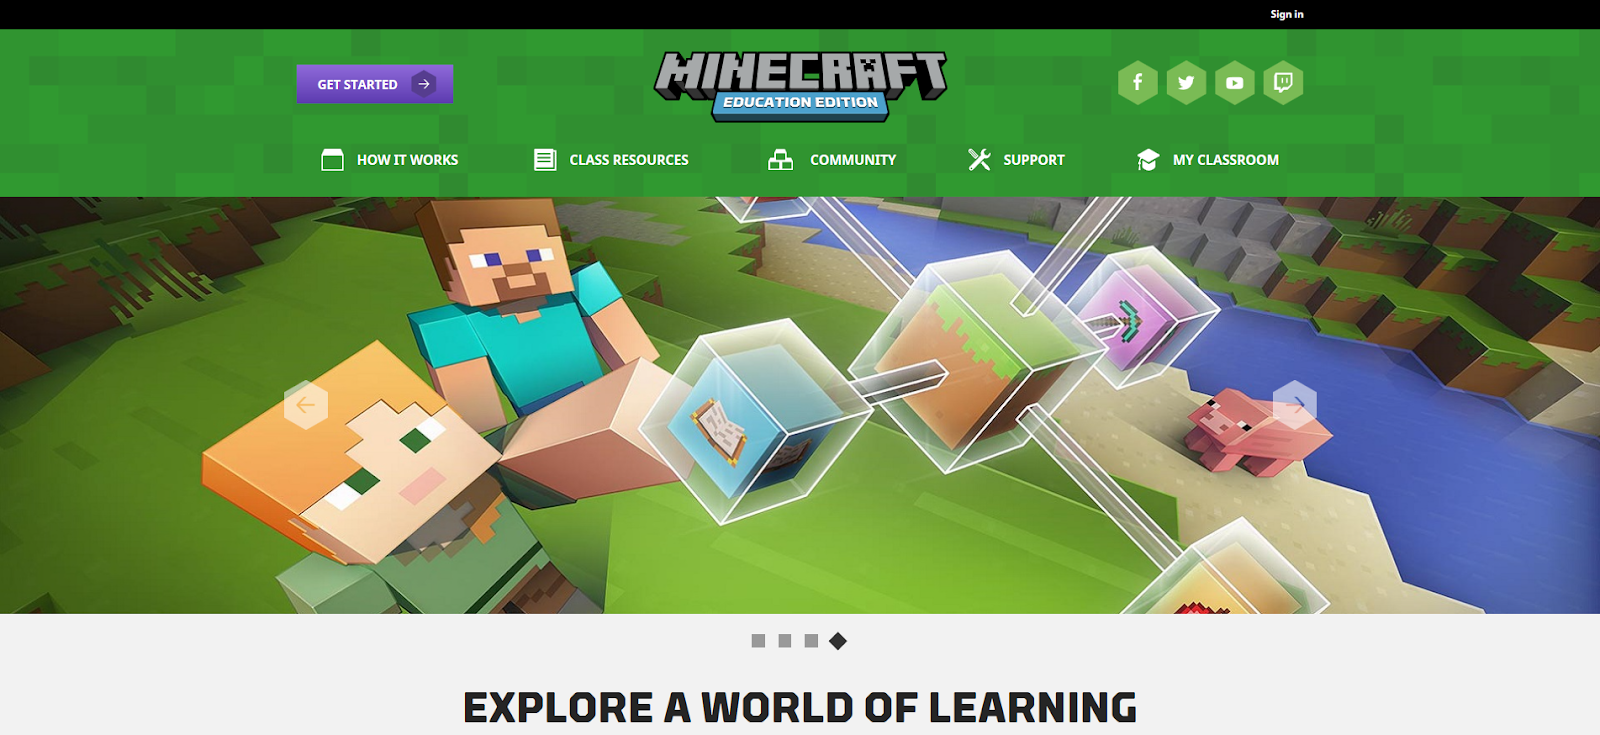
\includegraphics[width=\textwidth,height=\textheight,keepaspectratio]{images/Minecraft.png}
	\caption{Projekt Minecraft in Education}
	\label{projectMinecraft}
\end{figure}

Im Jahr 2009 wurde Minecraft (Version old aplha rd-132211) das erste mal vom
Studio Mojang veröffentlicht. Hauptentwickler war Markus Notch Persson. Zu Beginn wurde Minecraft
ausschließlich über die eigene Webseite des Studios vertrieben und löste bereits nach kurzer Zeit,
einen Hype in der Spielewelt aus. 
\cite{WikiMinecraft}

Minecraft ist ein Computerspiel ohne direktes Spielziel, man spricht von einem \textbf{Sandbox}-Spiel.
Der Spieler übernimmt die Kontroller über einen Avatar und kann mithilfe von würfelförmigen Blöcken,
in einer 3D-Welt Konstruktionen erschaffen oder vorhandene bearbeiten. Der Kreativität selbst,
sind dabei kaum Grenzen gesetzt, es gibt eine Vielzahl verschiedener Blockarten mit unterschiedlichen
Eigenschaften. So gibt es Blöcke die physikalisch Korrekt von der Schwerkraft beeinflußt werden,
andere die wiederrum in der Luft schweben können und manche die sich wie Flüssigkeiten verhalten.
\cite{WikiMinecraft}

Ein weiterer Grund für die fast unendlichen Möglichkeiten, ist die Erweiterbarkeit des Spiels durch
,von Spielern erstellten, Modifikationen (In der Szene Mods genannt). Mit diesen Erweiterungen ist es
möglich, bis auf das Blocksystem, alle Bereiche des Spieles anzupassen. Einem Weltraumspiel oder einer
Dreidimensionalen Murmelbahn steht nichts im Wege. Neue Arten von Blöcken mit neuen Eigenschaften lassen
sich dabei ebenso einfügen. Eine dieser Modifikationen ist das Projekt Minecraft in Education, welches
von Microsoft gefördert und Vertrieben wird, mit dem Ziel eine neue Generation von Lernspielen zu erschaffen.
